\section{Results}
The results are separated in three sections. First the fluxes from the three different methods are presented. Then, a comparison is made with the Chandra spectra from \cite{Dennerl2002DiscoveryChandra} and with the solar flux variation for the observation window. Finally, the solar event locator is presented.
    \subsection{Fluxes results}

    
    \textbf{22.04.2022}

    \textbf{Fig.} \ref{22_lc} shows the flux obtained with the different methods for the 22.04.2022. The colours of the different data points correspond to the different scws listed in \textbf{Tab.} \ref{journal} in that same order. As one wishes to combine the measurement of the fluxes with differing errors, a weighted average and uncertainty are computed in the following way:

    \begin{align}
        & \mu = \frac{\sum_i\frac{x_i}{\sigma_i^2}}{\sum_i \frac{1}{\sigma_i^2}} \\
        & \sigma(\mu) = \frac{1}{\sum_i\frac{1}{\sigma_i^2}}
    \end{align}

        \begin{figure}[H]
        \centering
        \begin{subfigure}{\textwidth}
            \centering
            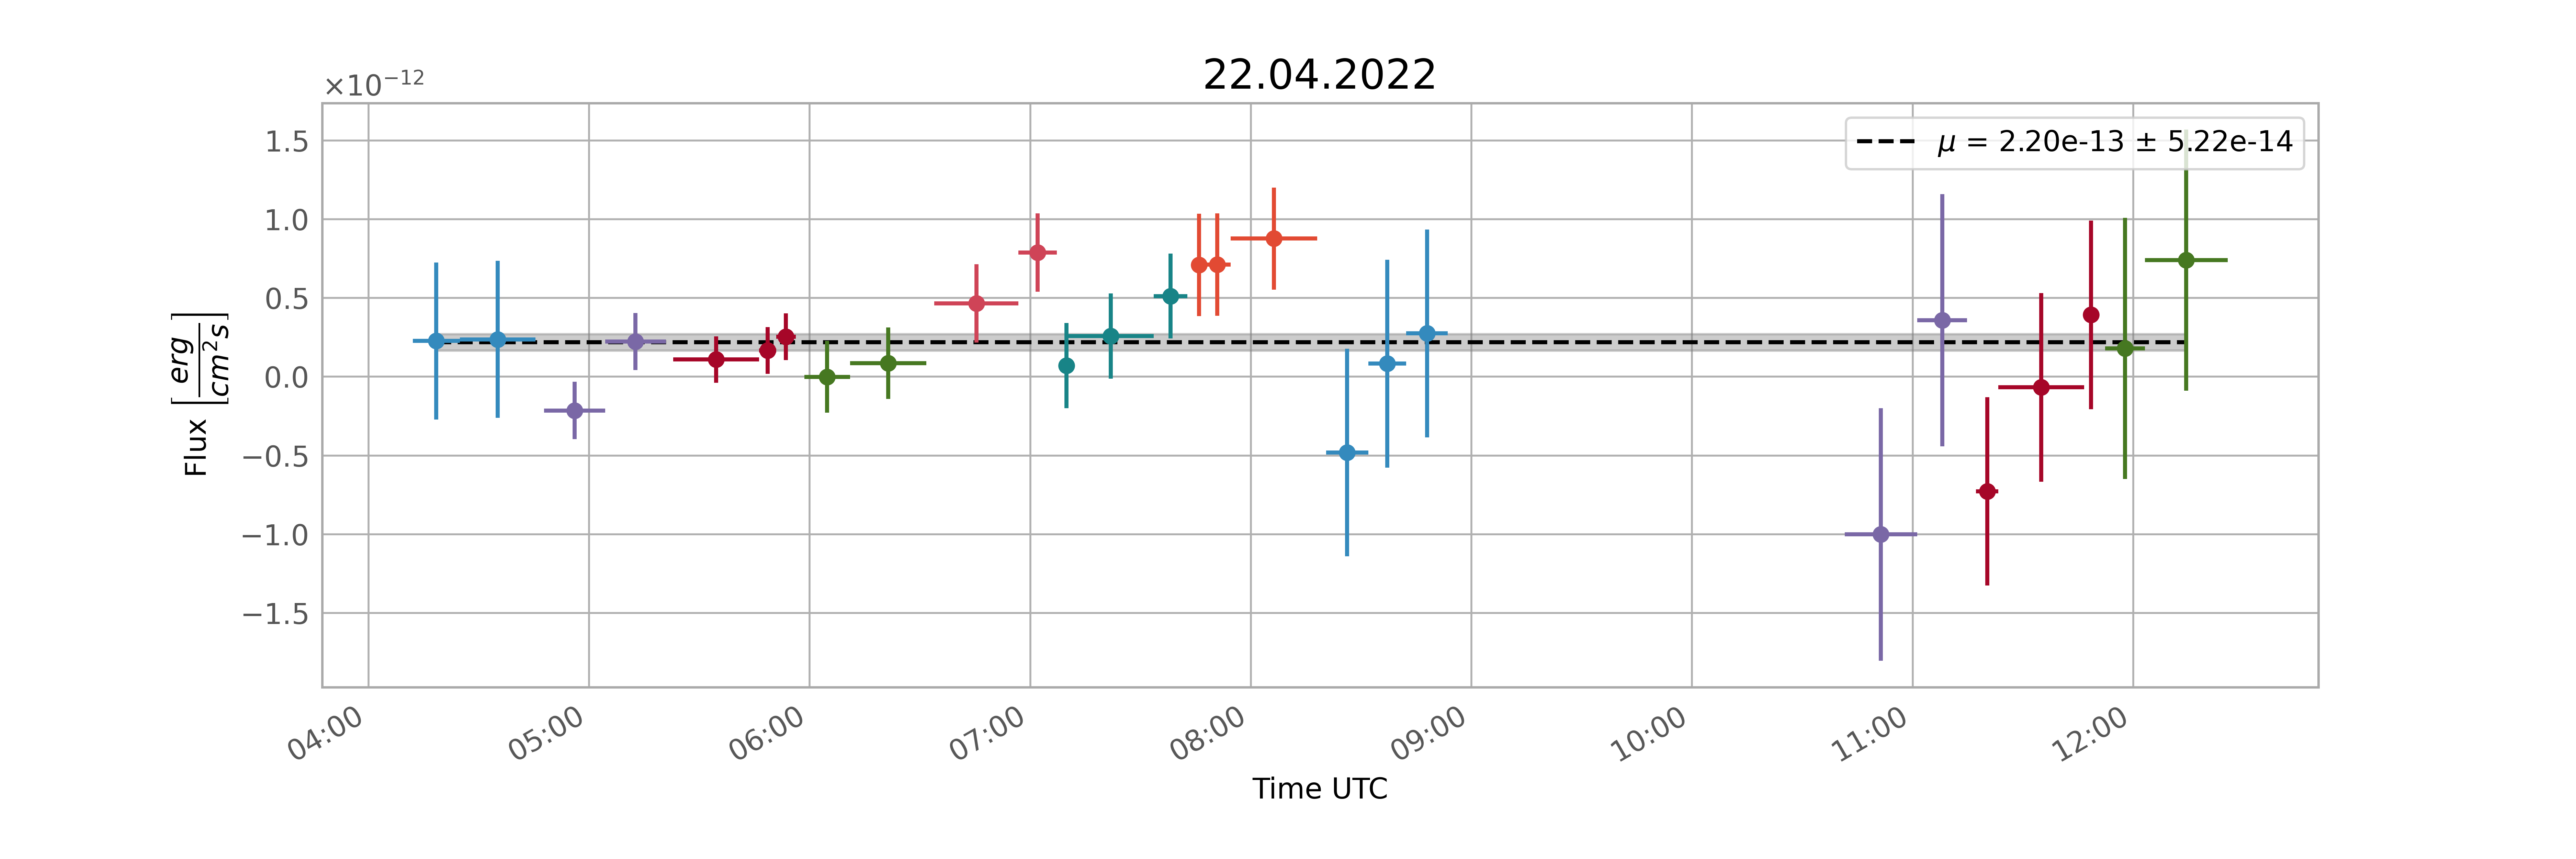
\includegraphics[width=0.8\textwidth]{report/Figures/results/lc_2204.png}
        \end{subfigure}%
        \hspace{1em}
        \begin{subfigure}{\textwidth}
            \centering
            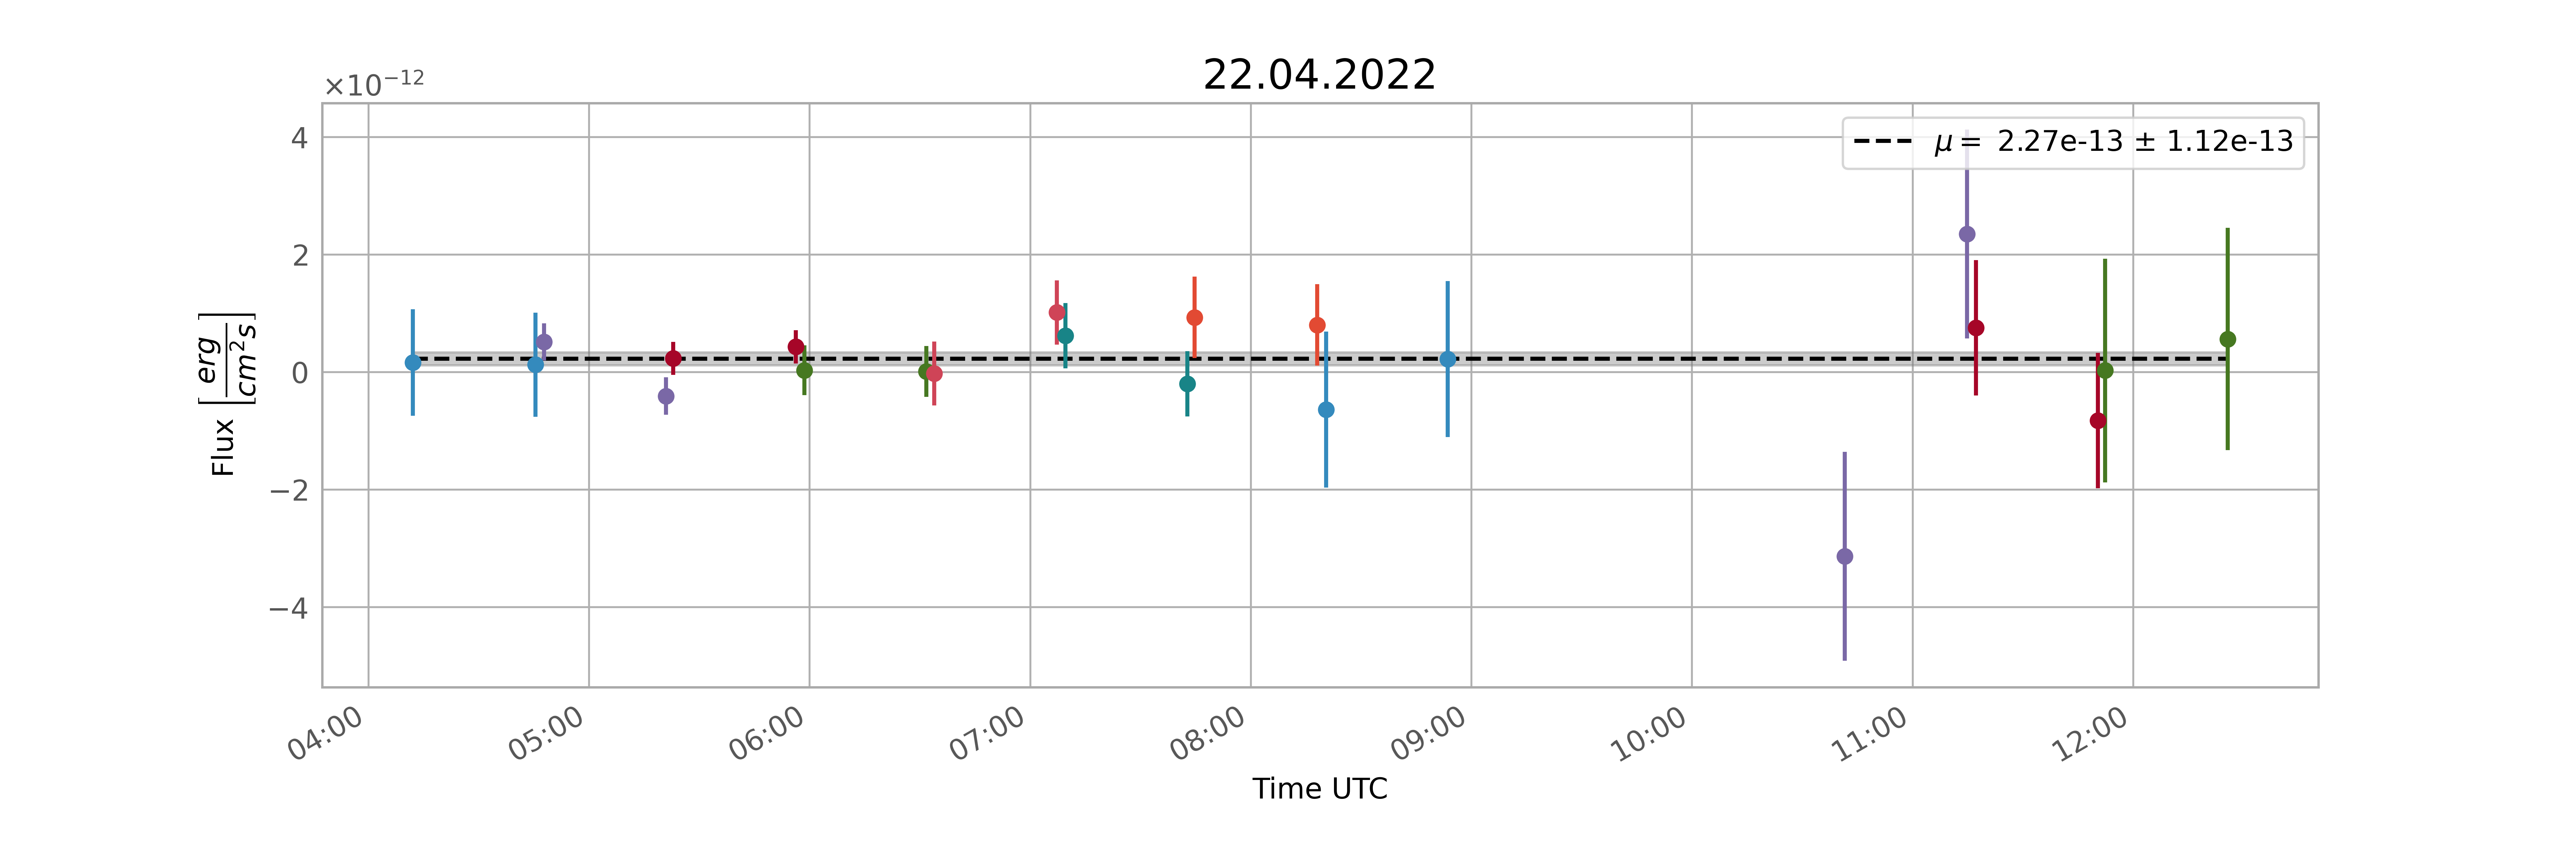
\includegraphics[width=0.8\textwidth]{report/Figures/results/lc_2204_psf_notconst.png}
        \end{subfigure}
        \hspace{1em}
        \begin{subfigure}{\textwidth}
            \centering
            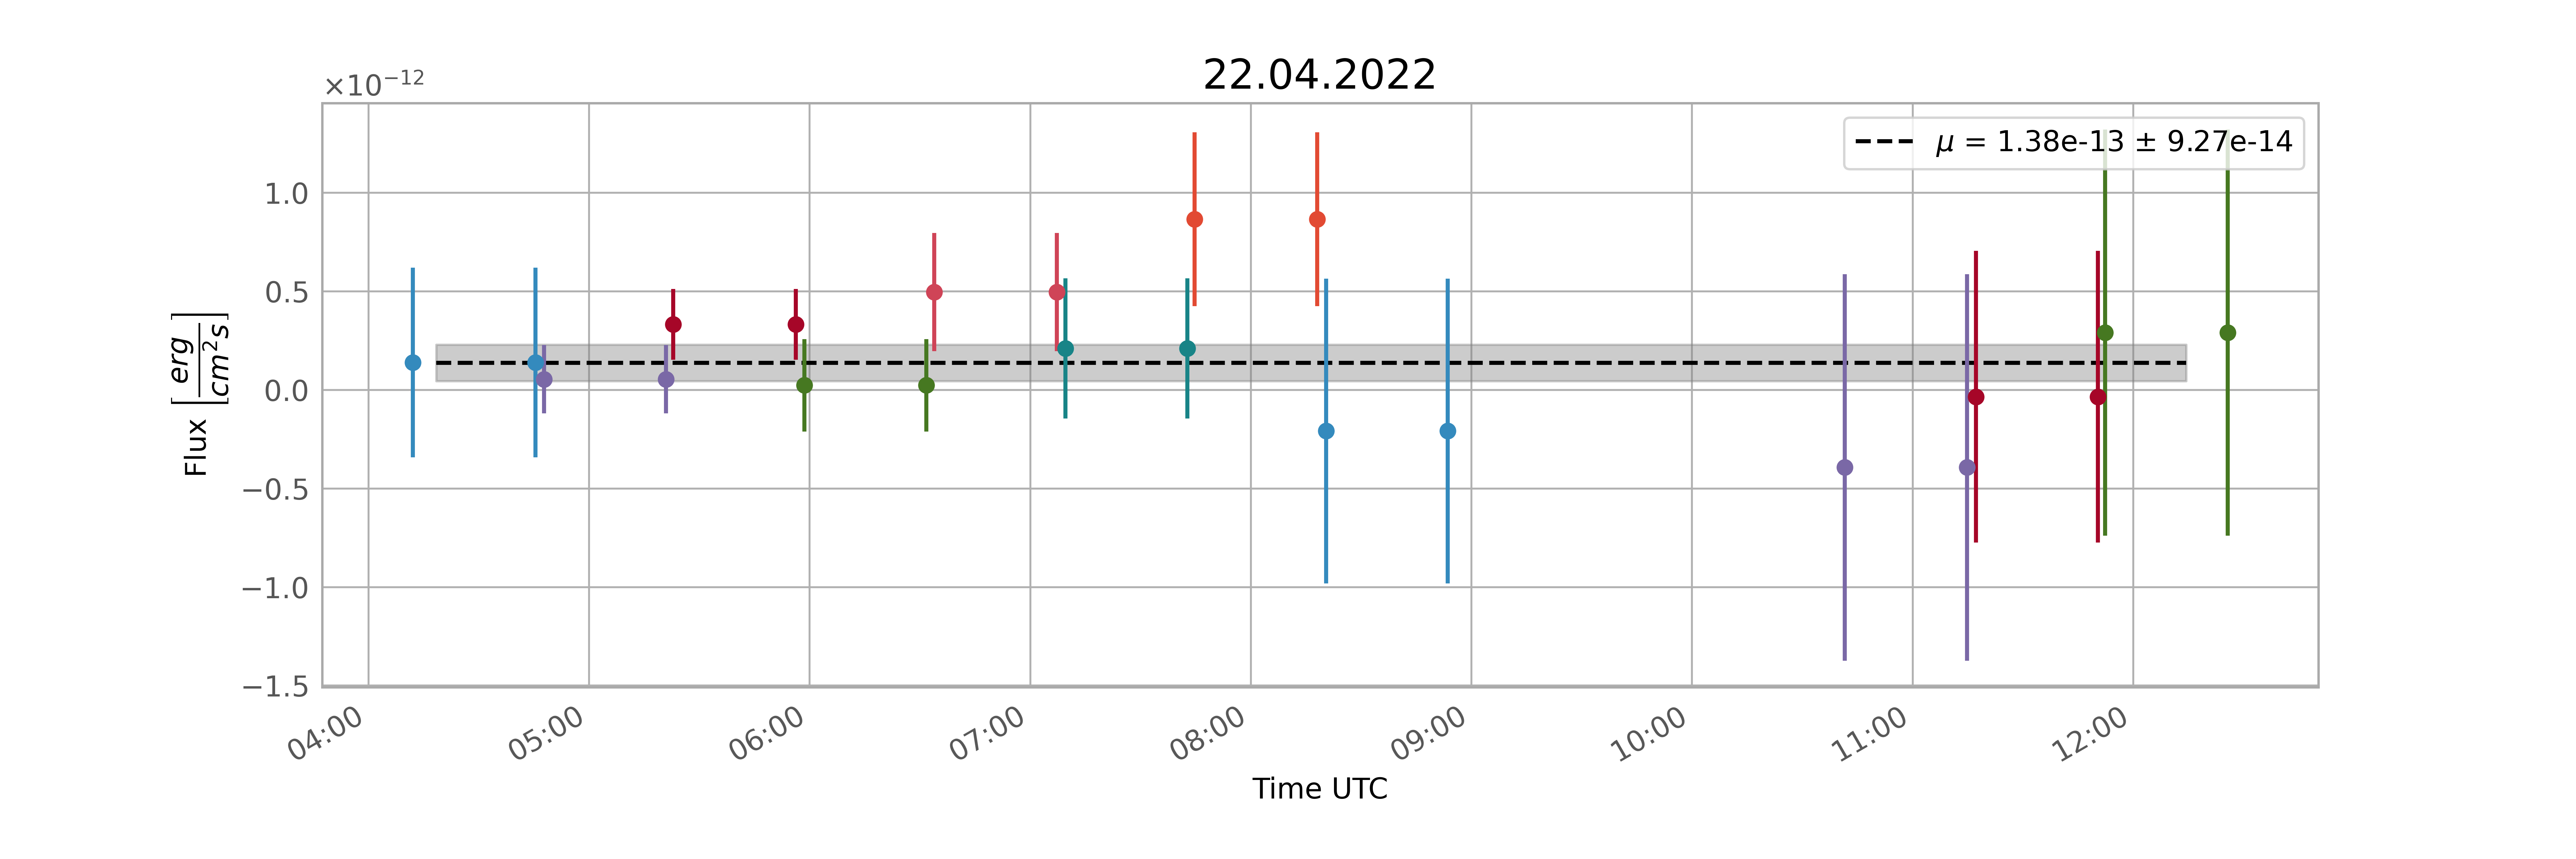
\includegraphics[width=0.8\textwidth]{report/Figures/results/lc_2204_psf_const.png}
        \end{subfigure}
        \caption{For the 22.04.2022, from top to bottom: LC using the pixel value, the non constant PSF model and the constant PSF model.}
        \label{22_lc}
        \end{figure}
        

    \paragraph{24.04.2022}

    The same is done with the 24.04 scws and is shown on \textbf{Fig.} \ref{24_lc}.
    
        \begin{figure}[H]
        \centering
        \begin{subfigure}{\textwidth}
            \centering
            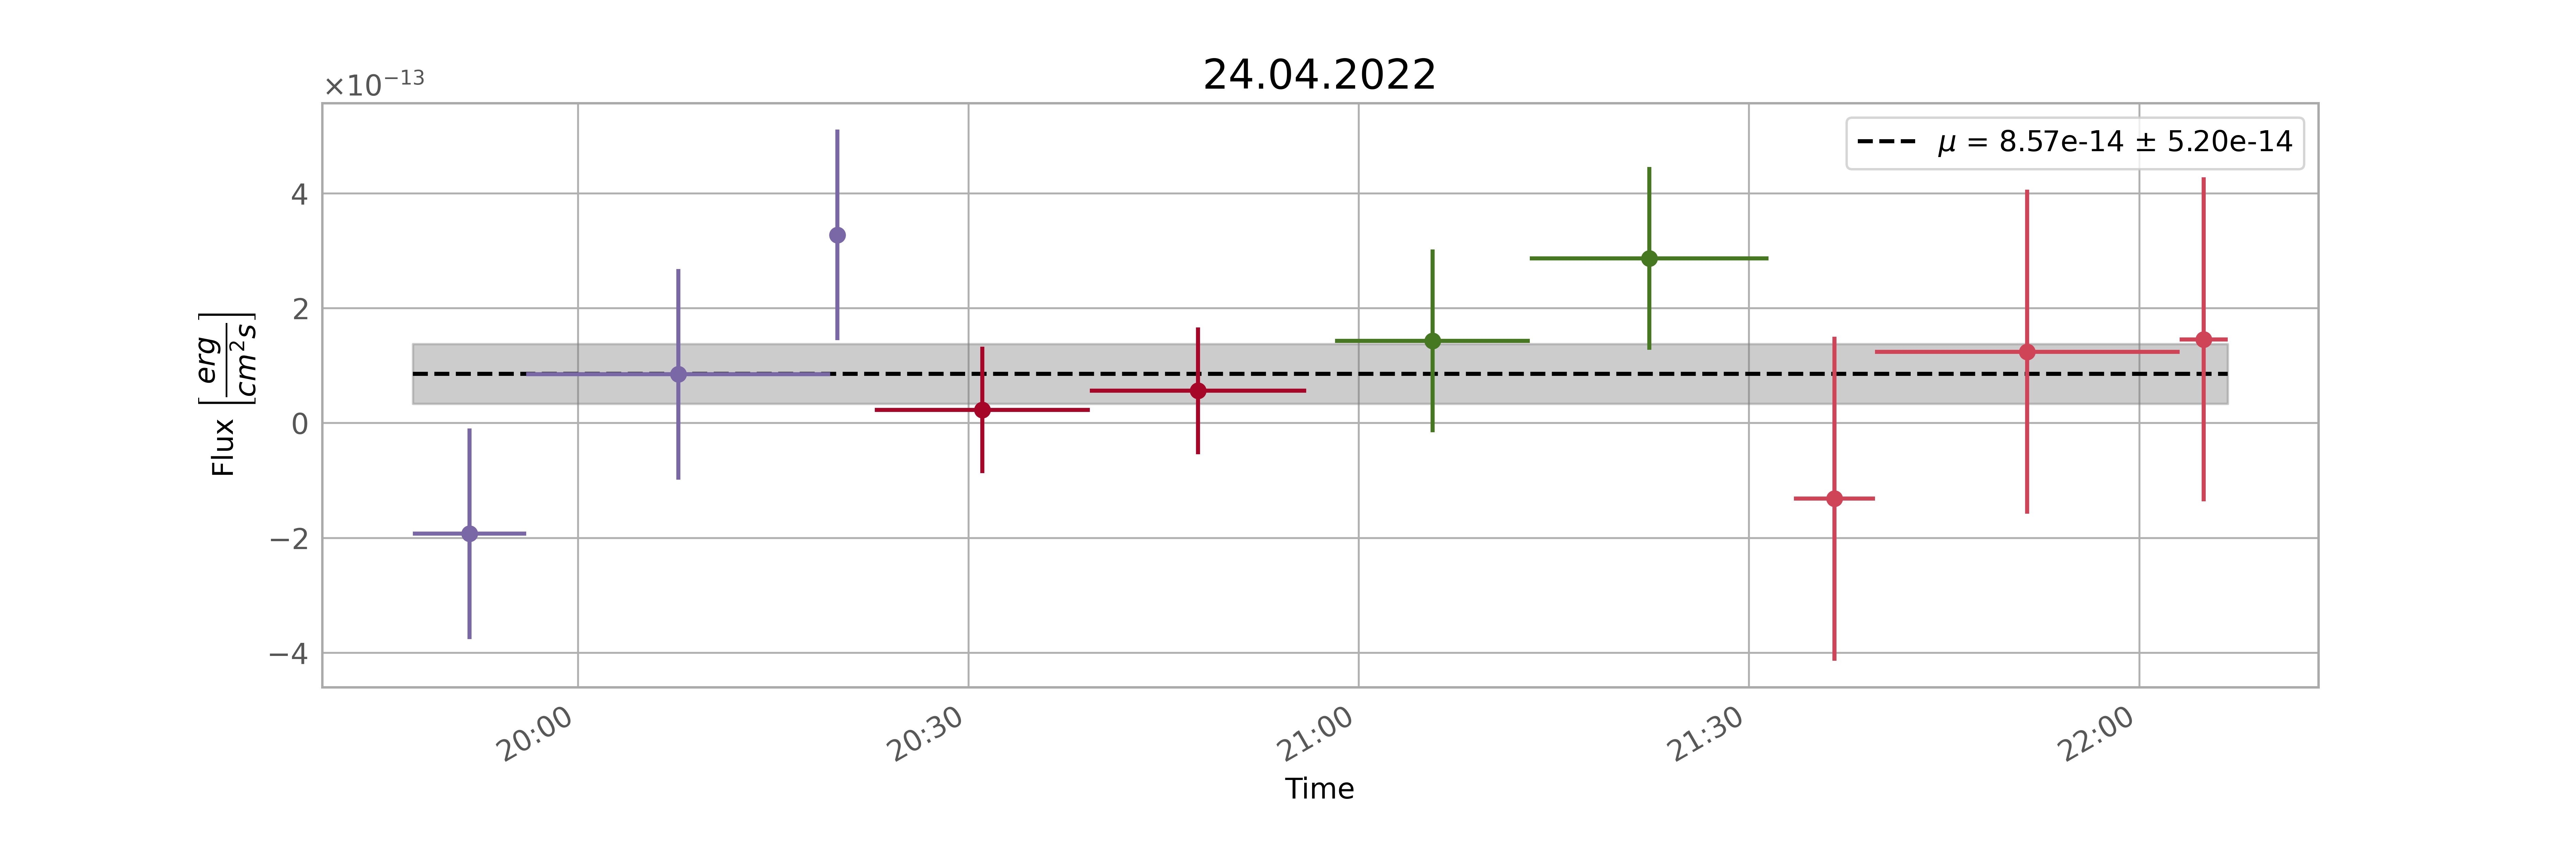
\includegraphics[width=0.8\textwidth]{report/Figures/results/lc_2404.png}
        \end{subfigure}%
        \hspace{1em}
        \begin{subfigure}{\textwidth}
            \centering
            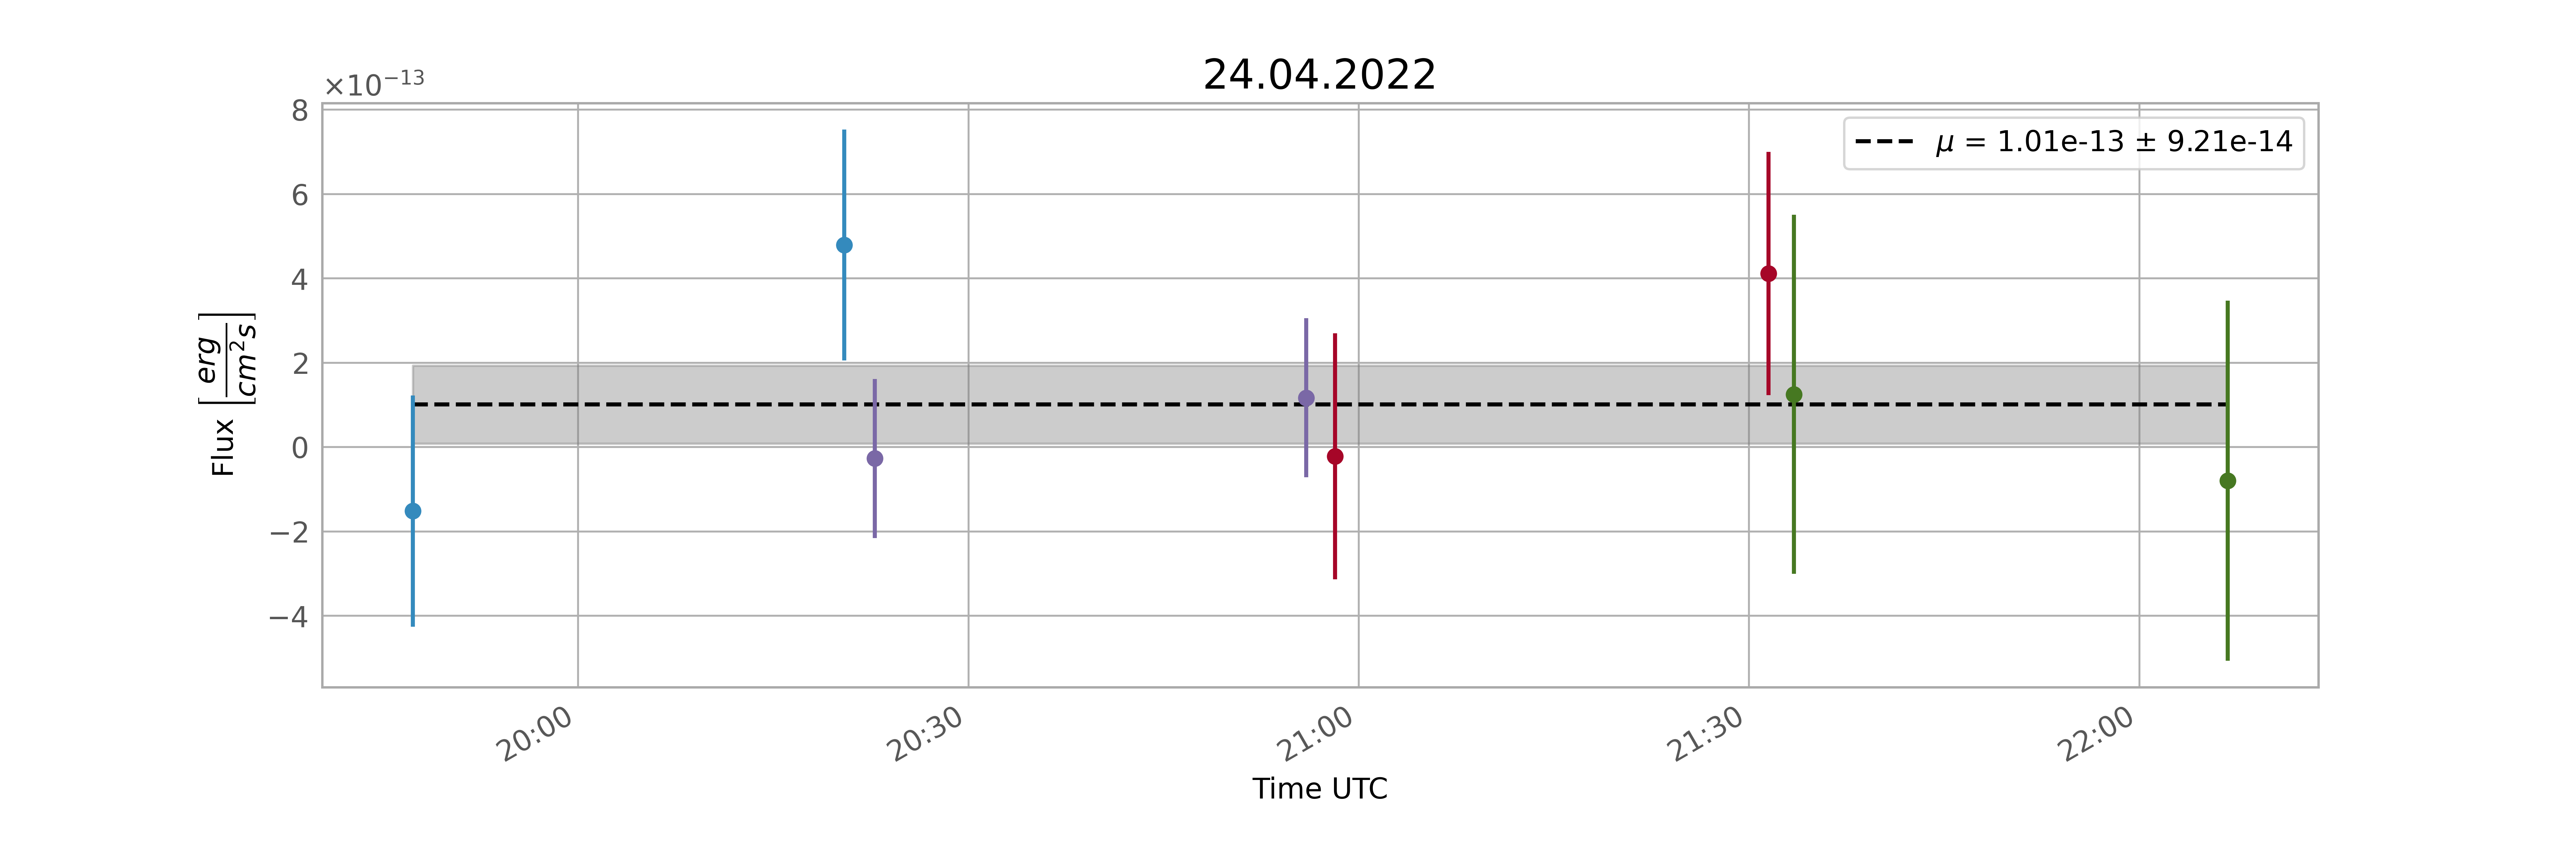
\includegraphics[width=0.8\textwidth]{report/Figures/results/lc_2404_notconst.png}
        \end{subfigure}
        \hspace{1em}
        \begin{subfigure}{\textwidth}
            \centering
            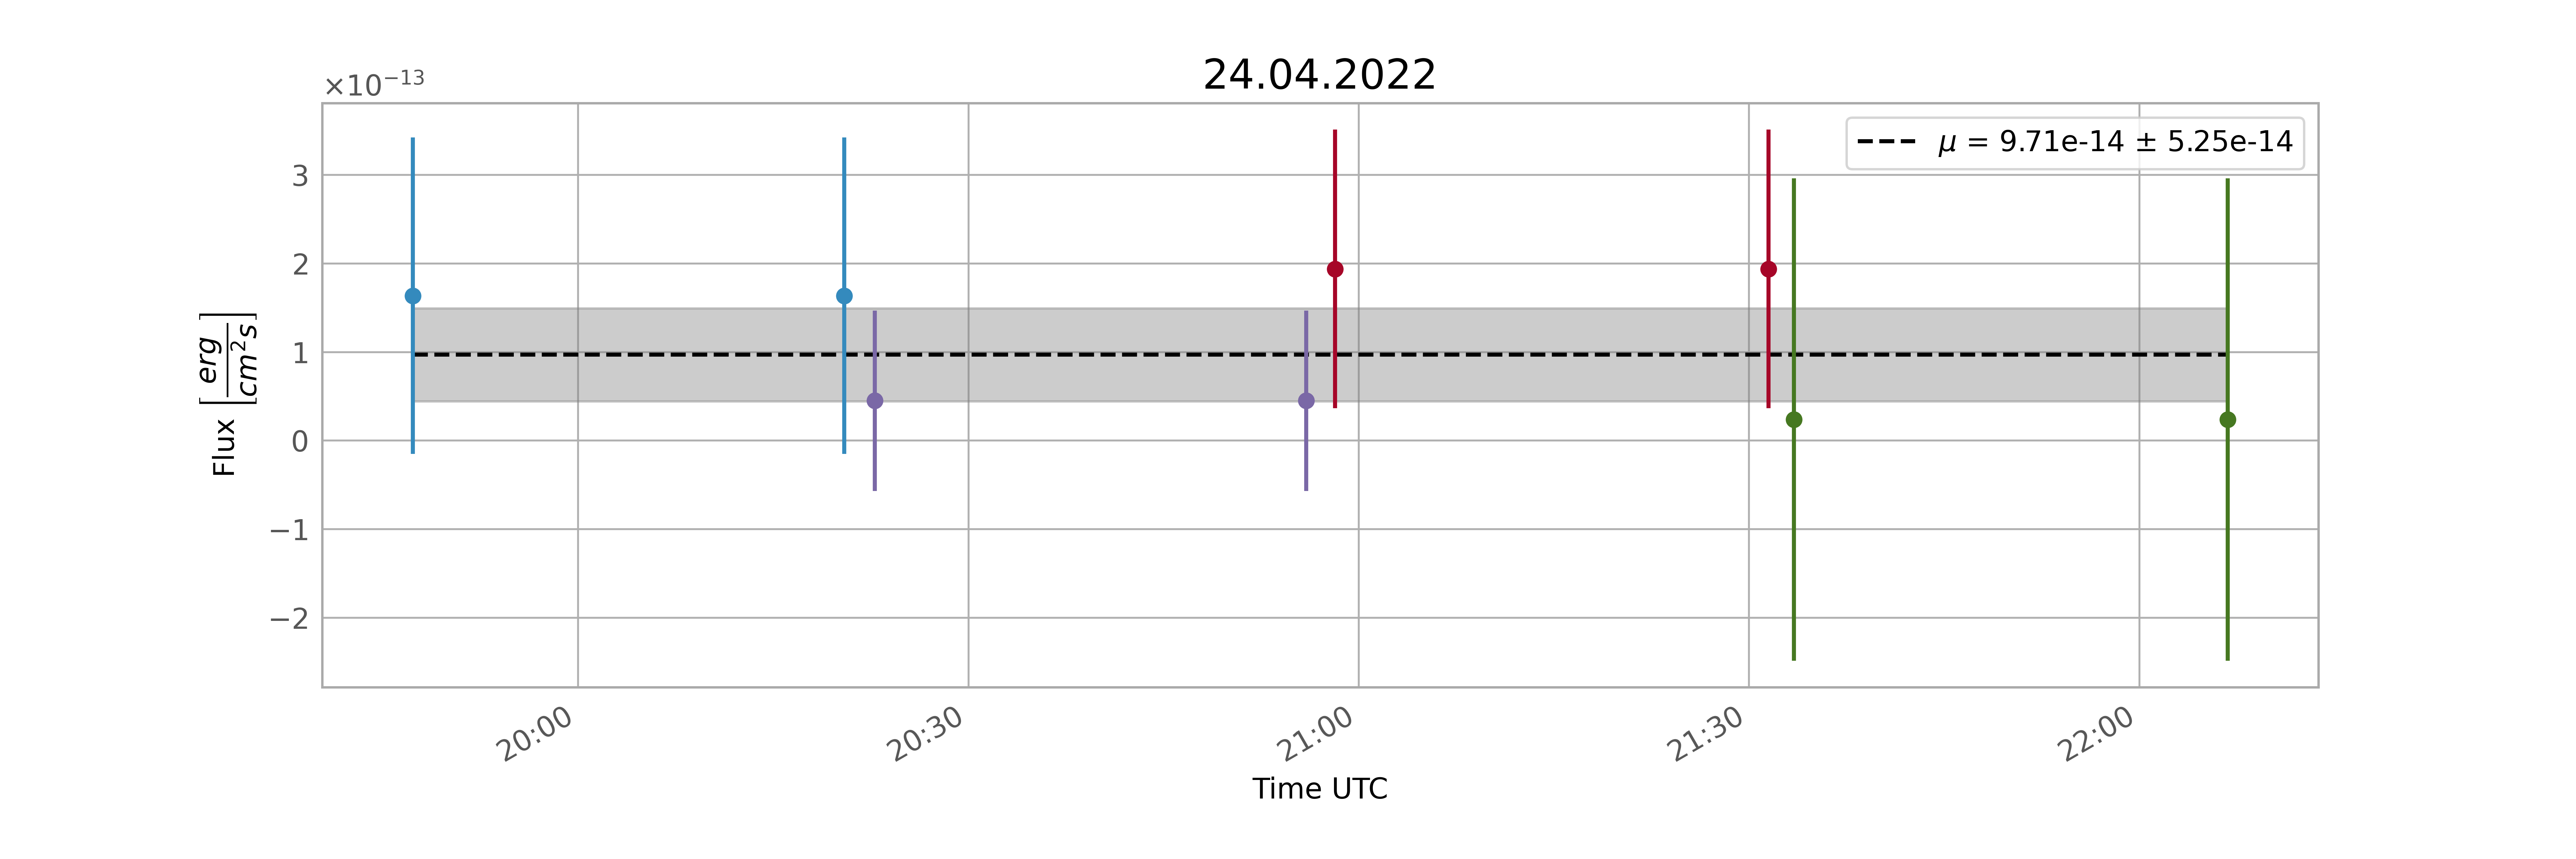
\includegraphics[width=0.8\textwidth]{report/Figures/results/lc_2404_psf_const.png}
        \end{subfigure}
        \caption{For the 24.04.2022, from top to bottom: LC using the pixel value, the non constant PSF model and the constant PSF model.}
        \label{24_lc}
        \end{figure}

    The average fluxes obtained with the first method for both windows are positive at the 3$\sigma$ level as per how JEM-X's variance map is built. For the other two methods, the fluxes are also positive given the 2\% threshold. Moreover, the values obtained between the three different methods are similar and reinforces the idea of a positive average flux observed in both windows.

    \begin{figure}[H]
        \centering
        \begin{subfigure}{0.42\textwidth}
            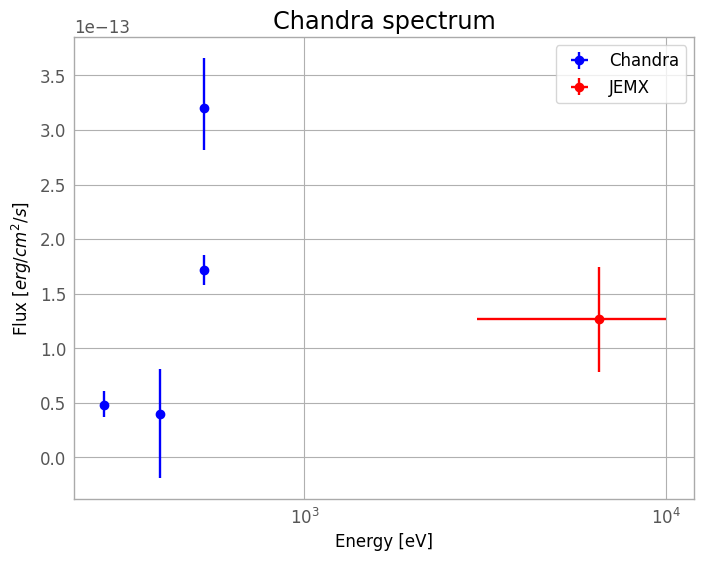
\includegraphics[width=\textwidth]{report/Figures/results/spectra_comp.png}
        \end{subfigure}%
        \hspace{1em}
        \begin{subfigure}{0.42\textwidth}
            \centering
            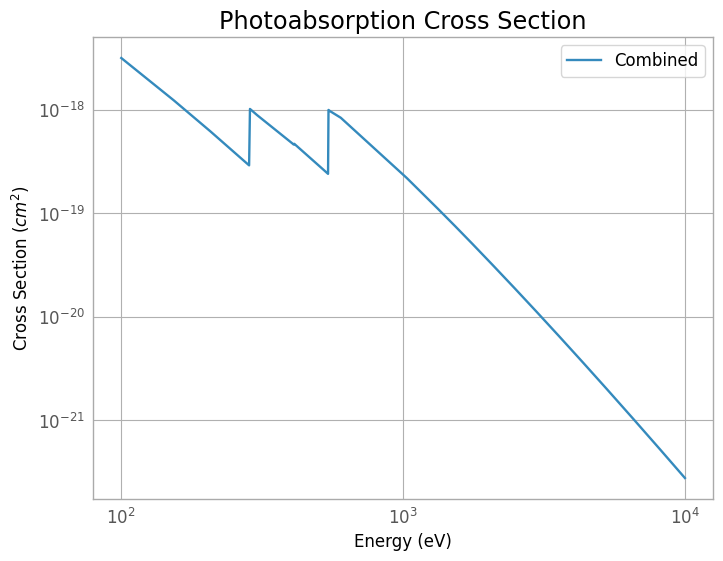
\includegraphics[width=\textwidth]{report/Figures/discussion/crosssection.png}
        \end{subfigure}
        \caption{(left) Comparison between the flux values obtained in \cite{Dennerl2002DiscoveryChandra} and this study. (right) Cross-section model for the Venusian atmosphere using the \texttt{Xraydb.sqlite} database.}
        \label{comp_spec}
    \end{figure}

    A comparison is made between the fluxes obtained in the \cite{Dennerl2002DiscoveryChandra} paper and here. The cross-section for fluorescence would suggest that the flux at higher energies should decrease. However, this is not the case here as shown on \textbf{Fig.} \ref{comp_spec}. This would suggest mainly two things: either the numbers are wrong in a way and do not represent correctly the flux from Venus or there are other physical sources apart from fluorescence that would contribute to Venus' luminosity in these higher energy ranges. For example, charge exchange interactions which could be more present in higher activity periods of the Sun\cite{BhardwajX-raysObjects}.
    
    \subsection{Concordance with solar flux variations}

    Given that the Sun's flux variability is of the order of minutes and that it is the main X-ray emitting cause on Venus, it is interesting to compare its time variability with Venus' which also varies on a timescale of minutes\cite{Dennerl2002DiscoveryChandra}. The GOES-16 solar flux at 1 A.U. in the XRSA channel is shown at the top of \textbf{Fig.} \ref{goes22} and \ref{goes_24}. The time of each scw is plotted using the same colour code as before on these graphs.
    \begin{figure}[H]
        \centering
        \begin{subfigure}{0.9\textwidth}
        \centering
            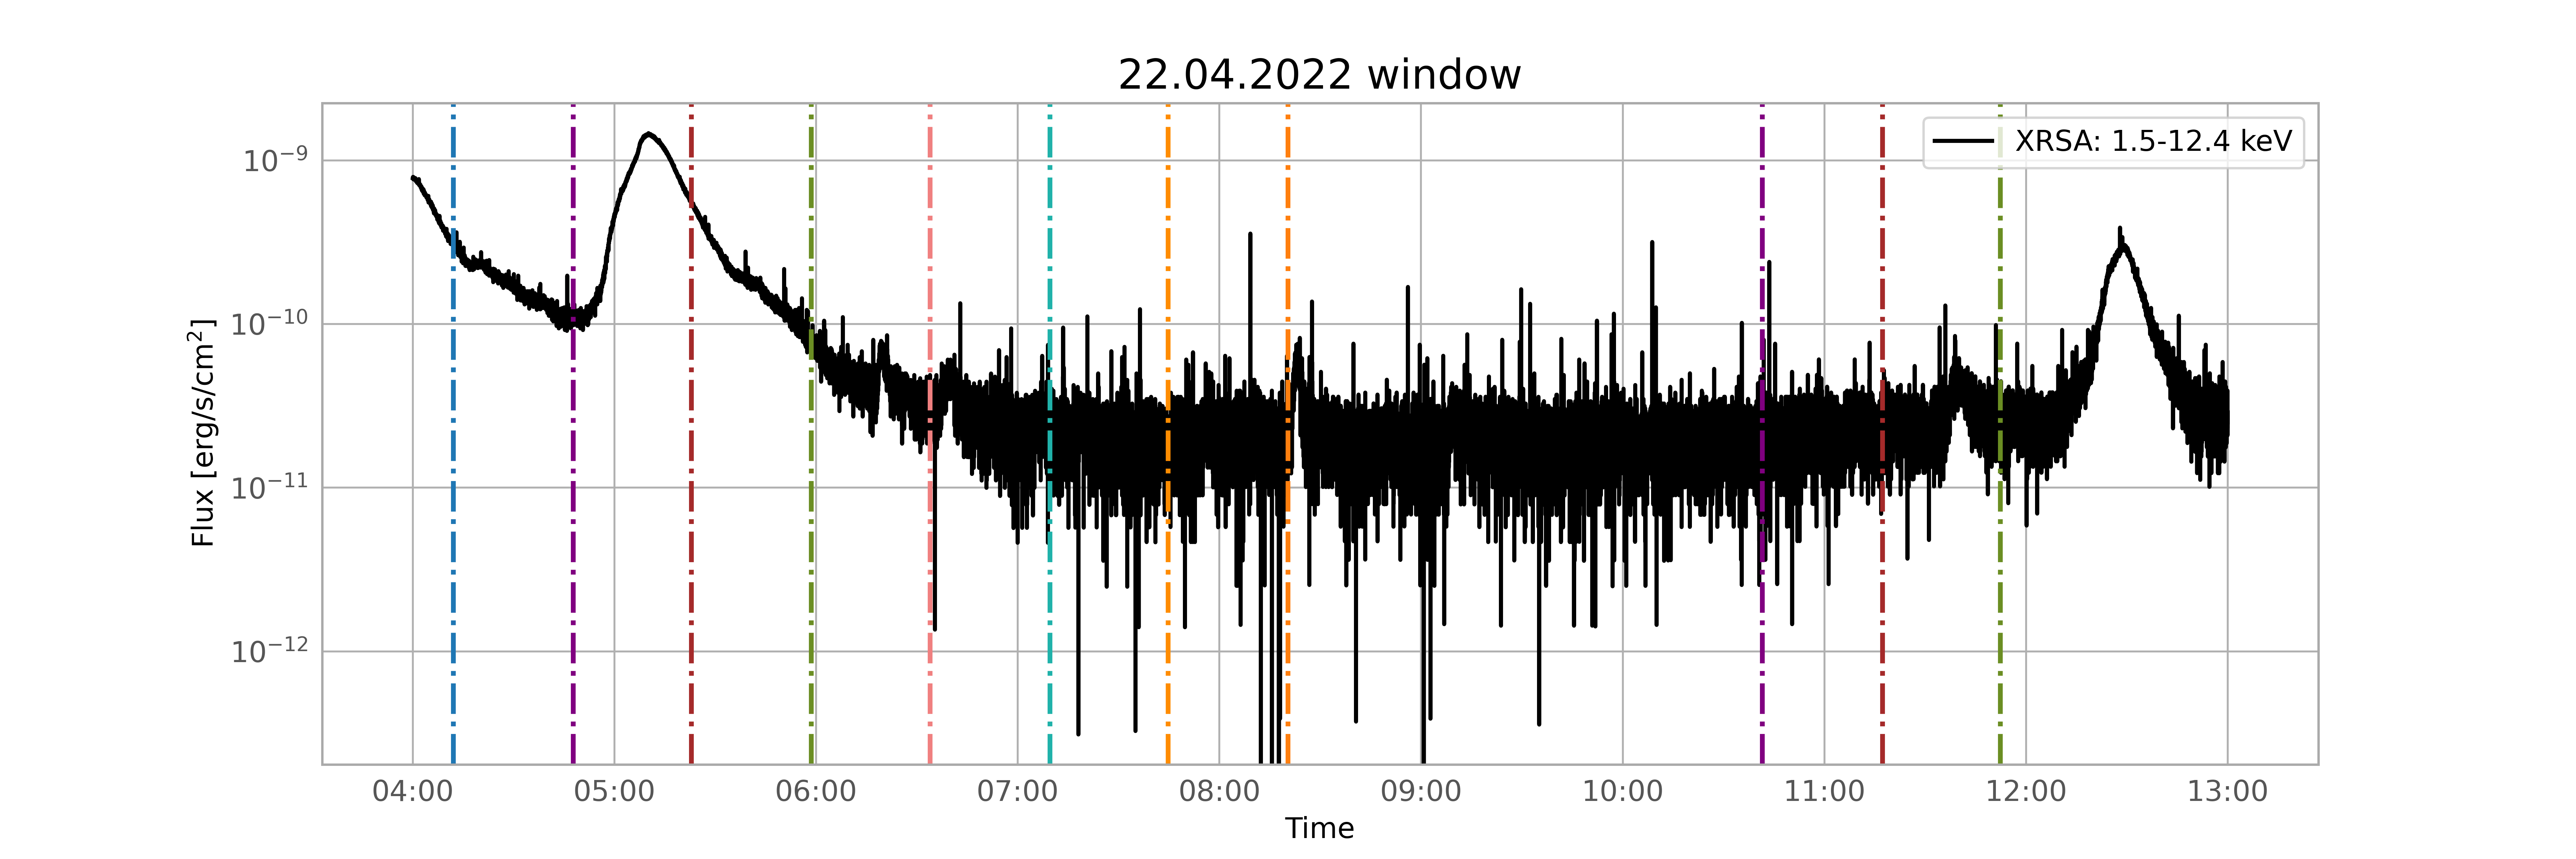
\includegraphics[width=\textwidth]{report/Figures/results/GOES_22.png}
        \end{subfigure}%
        \hspace{1em}
        \begin{subfigure}{0.75\textwidth}
            \centering
            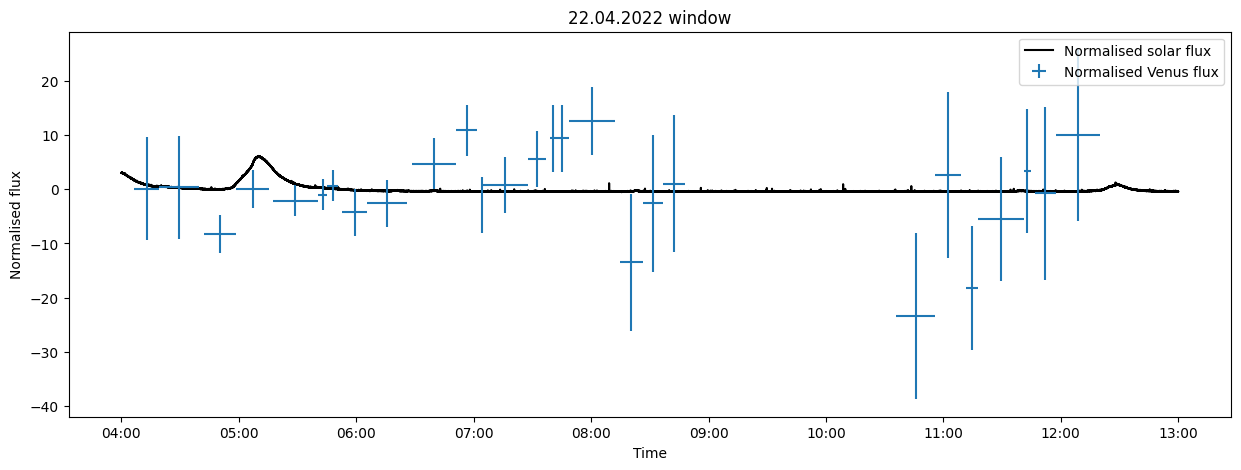
\includegraphics[width=\textwidth]{report/Figures/results/norm_22.png}
        \end{subfigure}
        \caption{Top: 22.04.2022 scws restricted view of the solar flux in the XRSA channel of GOES-16 overplotted with the times of the LC points.
        Bottom: Normalised solar and Venus fluxes plotted together. The data point times were corrected from light travel.}
        \label{goes22}
    \end{figure}


\begin{figure}[H]
    \centering
    \begin{subfigure}{0.9\textwidth}
        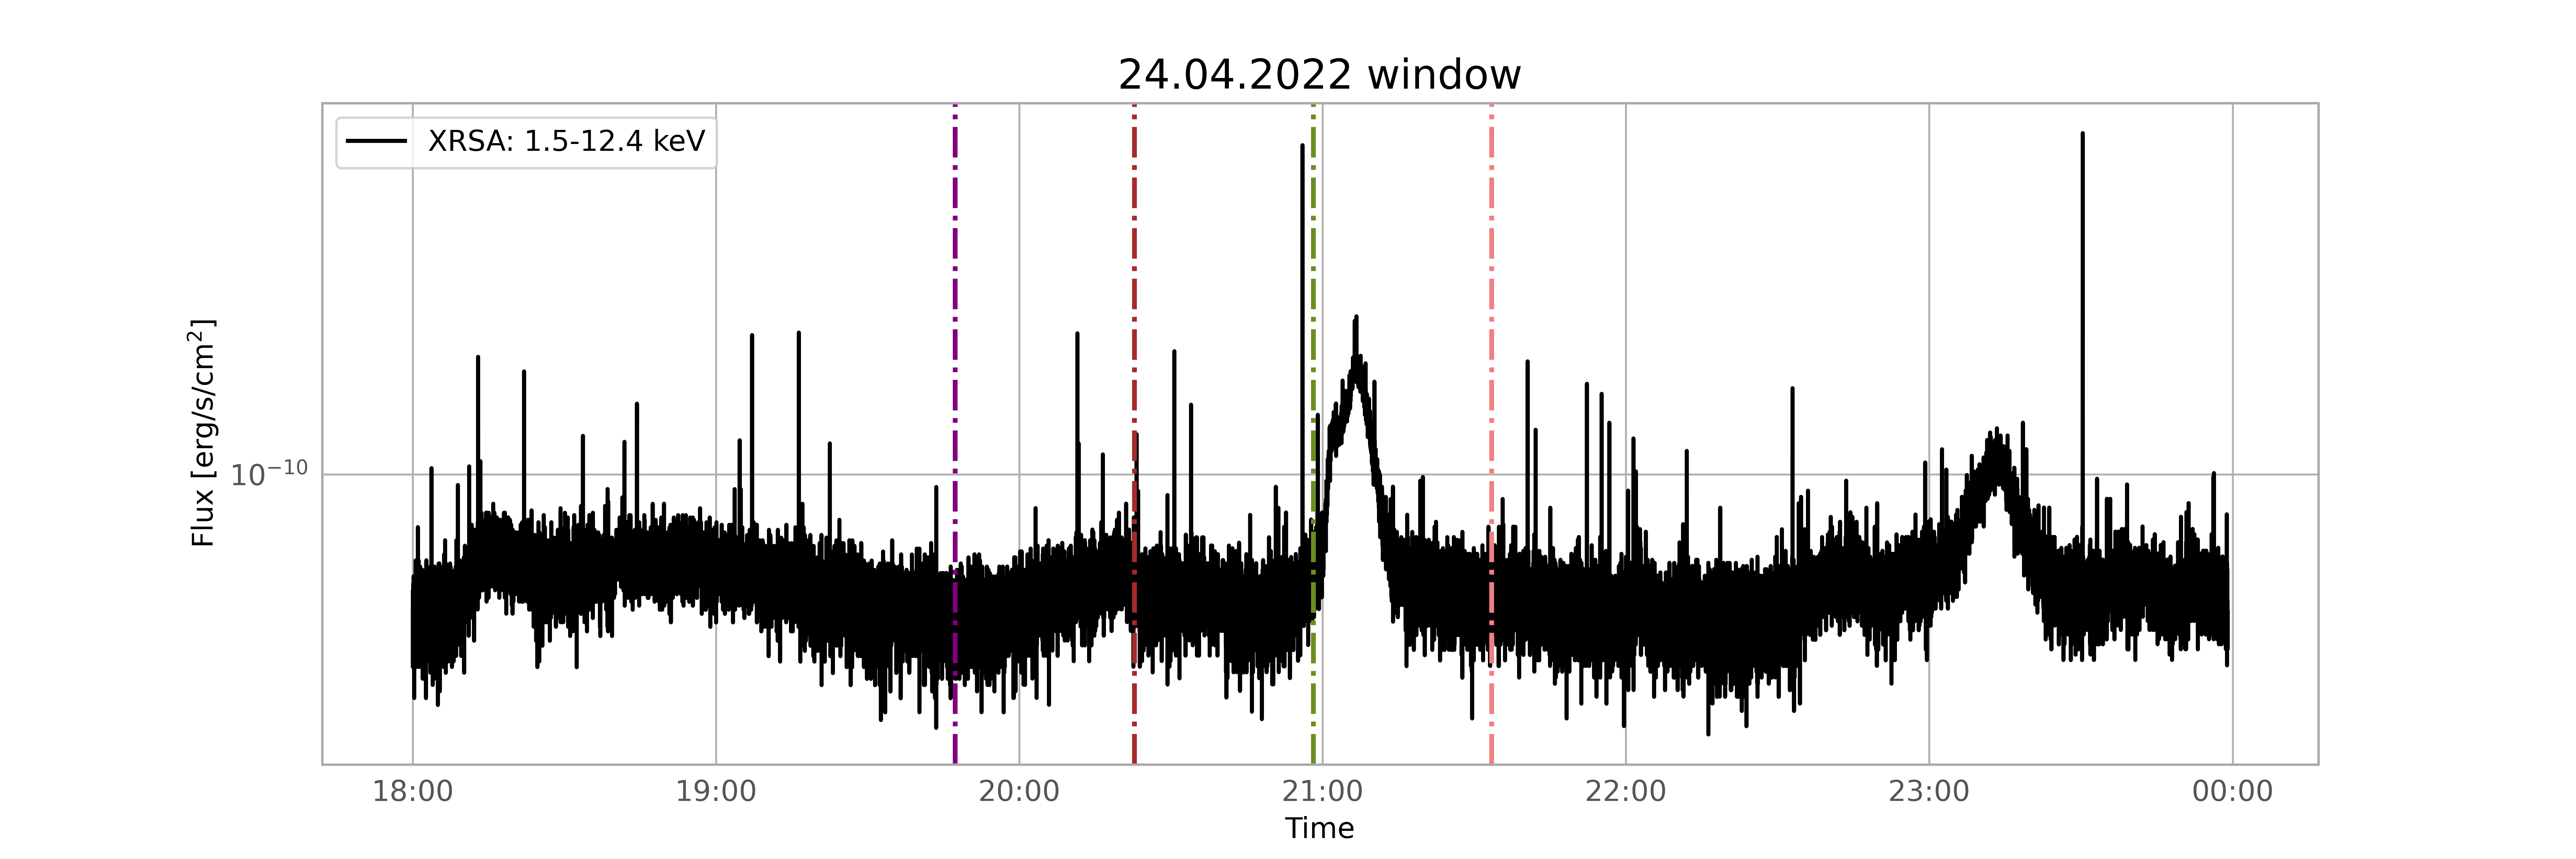
\includegraphics[width=\textwidth]{report/Figures/results/GOES_24.png}
    \end{subfigure}%
    \caption{Top: 24.04.2022 scws restricted view of the solar flux in the XRSA channel of GOES-16 overplotted with the times of the LC points.}
    \label{goes_24}
\end{figure}

\begin{figure}[H]
    \ContinuedFloat
    \centering
    \begin{subfigure}{0.75\textwidth}
        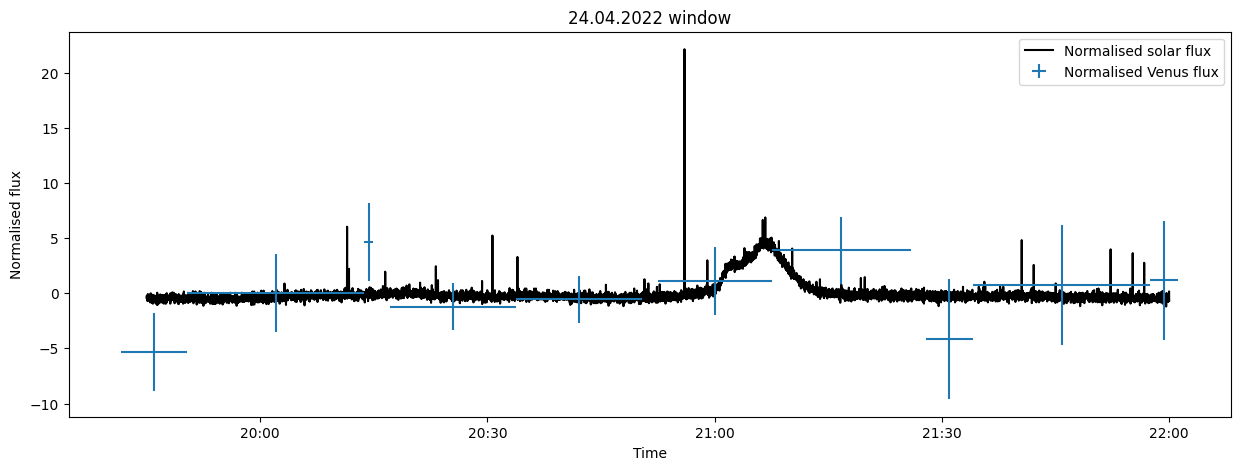
\includegraphics[width=\textwidth]{report/Figures/results/norm_24.png}
    \end{subfigure}
    \caption*{(continued) Bottom: Normalised solar and Venus fluxes plotted together. The data point times were corrected from light travel.}
\end{figure}

Moreover, Venus flux and the solar flux are normalised and plotted together on the bottom side of \textbf{Fig.} \ref{goes22} and \ref{goes_24}. The idea here is to inspect the time correlation between both quantities.  The data points were corrected from light travel time. For the solar flux, the path is: Sun $\rightarrow$ Earth. For the Venus flux, it is: Sun $\rightarrow$ Venus $\rightarrow$ Earth. The data points are 5.6 minutes late on the solar flux data. A two-sample Kolmogorov-Smirnov test is performed on these sample. The significance level is set at a standard 5\%. The results are p-values of 2.6\% and 4.8\% for respectively the 22.04.2022 and the 24.04.2022 windows.

The estimated average energy deposited on Venus in X-ray from the first scw to the last for each day and for the three different methods is given by: 

\begin{equation}
    E = \frac{\pi r_{\venus}^2\mu \Delta t}{illumination},
\end{equation}
where $r_{\venus}$ is Venus' radius and $\Delta t$ is the duration from the first scw to the last on one of the two days observed. The results are the following:

\begin{table}[H]
\centering
\begin{tabular}{@{}lcc@{}}
\toprule
\textbf{Method/Date}             & 22.04.2022    & 24.04.2022     \\ \midrule
Duration [s]                     & 29618         & 8370           \\
Pixel value [$10^{16}$ erg]      & 1.15 $\pm$ 0.27 & 0.13 $\pm$ 0.077 \\
Constant PSF [$10^{16}$ erg] & 0.72 $\pm$ 0.14 & 0.14 $\pm$ 0.077 \\
Non-constant PSF [$10^{16}$ erg]     & 1.18 $\pm$ 0.58 & 0.15 $\pm$ 0.13  \\ \bottomrule
\end{tabular}
\caption{Estimated energy deposited on Venus given the three flux methods.}
\label{depo}
\end{table}

The results all overlapped except for the 22.04.2022 window with the constant PSF method.

    % talk about estimated energy deposited on venus too.
    
    \subsection{Solar events locations}
    The direction of propagation of the solar flares and CMEs are estimated in the HGS thanks to the HEK data based on the HPC coordinates given by the GOES satellite for the flares and the LASCO instrument on SOHO for the CMEs. The model is as simplistic as it can get but it is a first try at such as estimation. A line is drawn between the centre of the Sun and the surface coordinates of the event. The results are shown on \textbf{Fig.} \ref{locator}. The events' directions are clearly biased and this is discussed in the next section. 
    
    \textbf{Fig.} \ref{Mclass_flare} shows an image of the M1.1 class flare detected as the first peak on the 22.04.2022 solar flux plot on \textbf{Fig.} \ref{goes22} by the AIA imager.

        \begin{figure}[H]
        \centering
        \begin{subfigure}{.47\textwidth}
            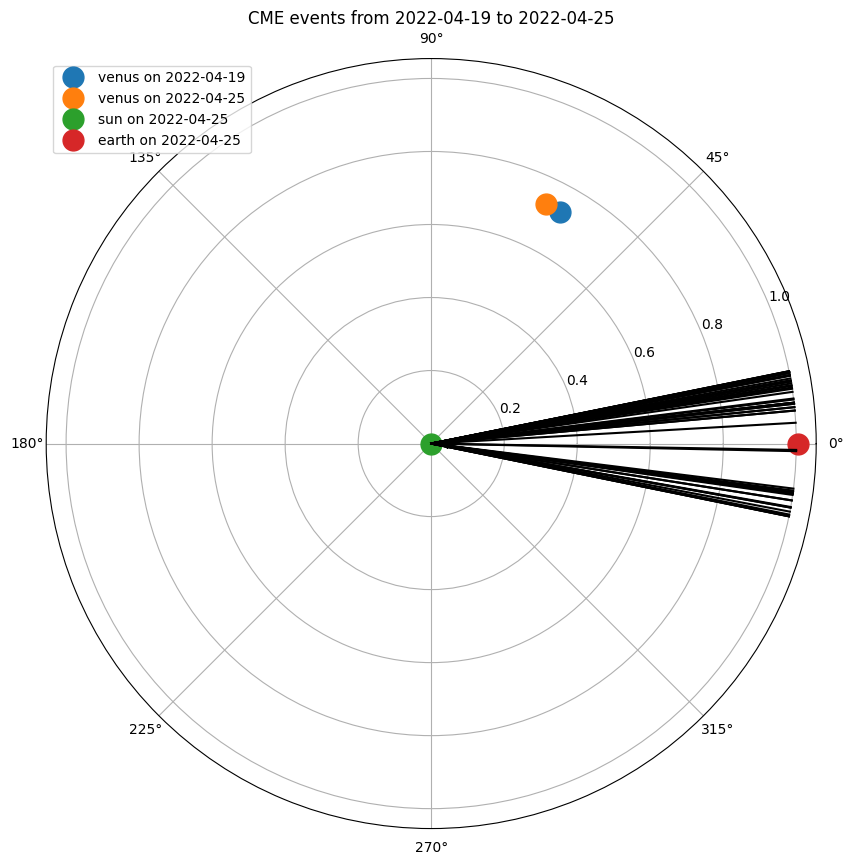
\includegraphics[width=\textwidth]{report/Figures/results/cme_loc.png}
        \end{subfigure}%
        \hspace{1em}
        \begin{subfigure}{.47\textwidth}
            \centering
            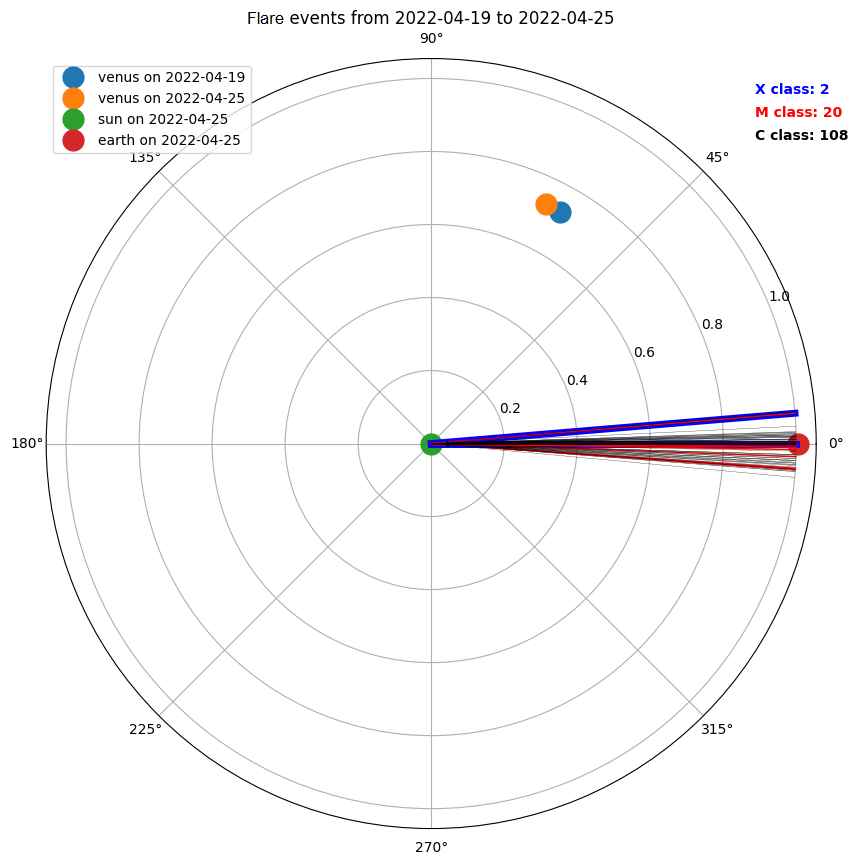
\includegraphics[width=\textwidth]{report/Figures/results/fl_loc.png}
        \end{subfigure}
        \caption{For the 19.04.2022 to 25.04.2022 period: (left) Propagation directions of all CMEs contained in the HEK. (right) Propagation directions of all flares contained in the HEK. The classes of the flares and numbers are indicated in colors.}
        \label{locator}
        \end{figure}

    \begin{figure}[H]
        \centering
        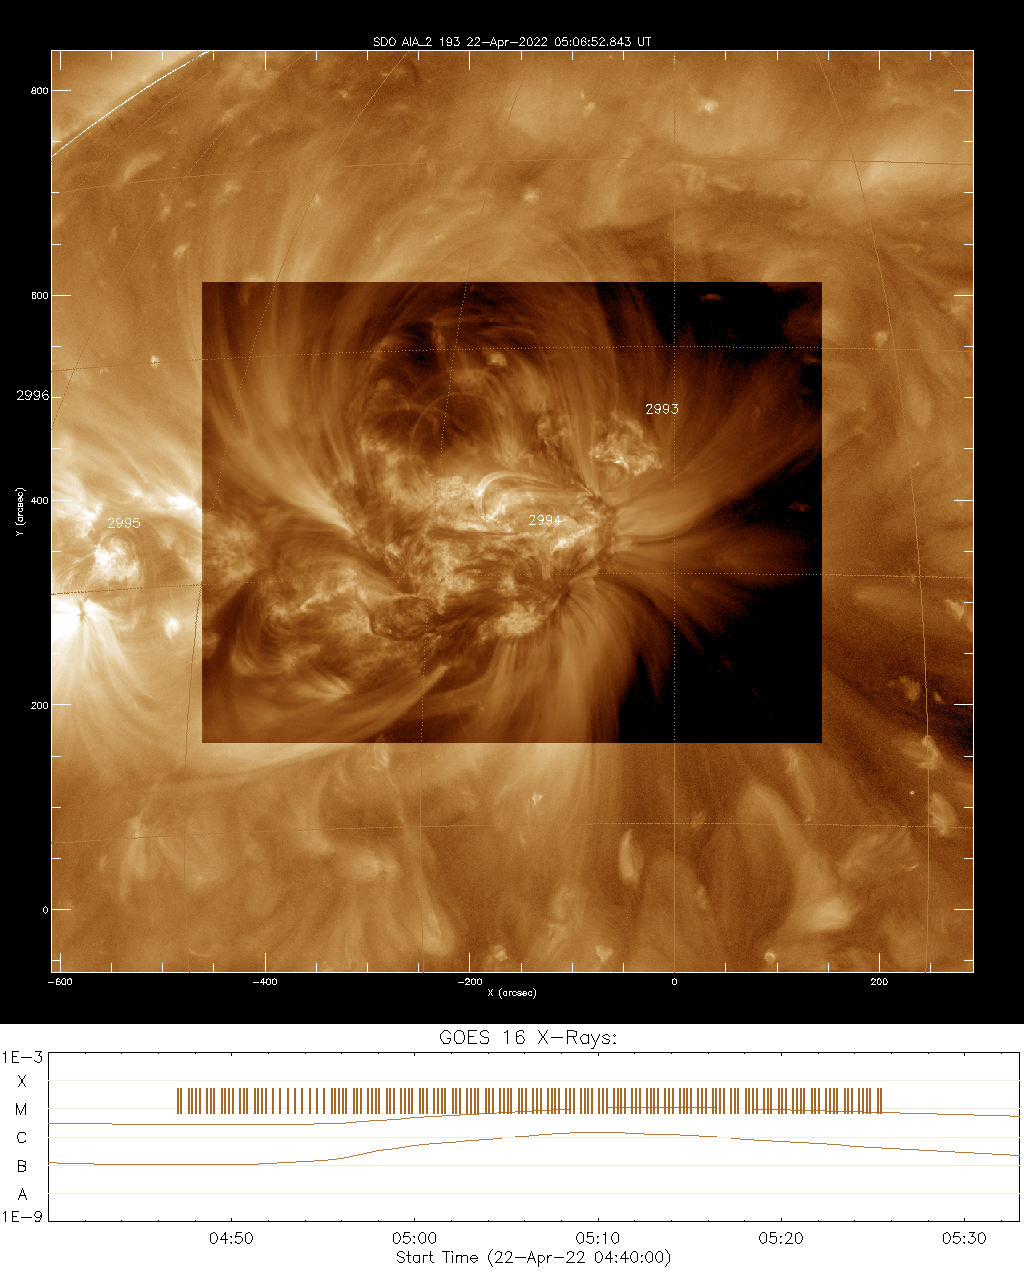
\includegraphics[width = 10cm]{report/Figures/results/aia_Mclass_2204.png}
        \caption{AIA image of the M1.1 class flare visible in the 22.04.2022 window.}
        \label{Mclass_flare}
    \end{figure}